\section{Langkah-Langkah Percobaan}
\subsection{Persiapan Alat dan Bahan}
Sebelum memulai praktikum ini, praktikan mempersiapkan beberapa alat dan bahan yang diperlukan. Alat dan bahan yang praktikan bawa sendiri diantaranya, laptop yang sudah terinstall Winbox, dan kabel UTP. Sedangkan alat dan bahan yang telah disediakan adalah 1 set router mikrotik. Pengambilan dilakukan oleh perwakilan kelompok.

\subsection{Connecting Kabel}
Praktikan menghubungkan ether 1 dari router ke kable Internet ITS dan ether 7 ke laptop.

\subsection{Konfigurasi VPN PPTP}
\begin{enumerate}
  \item Login dan Reset Router \\
  Sebelum memulai konfigurasi, praktikan login dan mereset terlebih dahulu router yang akan digunakan agar tidak terjadi konflik ketika konfigurasi nanti. Kemudian, praktikan login ulang.
  \item Konfigurasi DHCP Client \\
  Agar bisa mendapatkan koneksi internet, router disetting untuk menerima DHCP. Untuk melakukannya, praktikan memilih menu IP > DHCP Client > +. Praktikan memilih ether 1 kemudian mencentang pilihan "Use Peer DNS" dan "Use Peer NTP". Terakhr pilih apply. Hasil dapat dilihat pada gambar \ref{fig:dhcp-client}
  \item Konfigurasi NAT \\
  Agar perangkat lokal dapat terhubung ke internet juga, NAT perlu dikonfigurasikan. Untuk melakukannya, praktikan memilih IP > Firewall  kemudian ke tab NAT > +.Praktikan mengisikan konfigurasi sesuai dengan modul kemudian pilih apply. Hasil dapat dilihat pada gambar \ref{fig:nat}
  \item Konfigurasi IP Lokal \\
  Pada ether 7, praktikan mengkonfigurasikan alamat lokal 192.168.10.2/24. Hasil dapat dilihat pada gambar \ref{fig:ip}
  \item Kofigurasi DHCP Server Lokal \\
  Praktikan melakukan konfigurasi DHCP server untuk ether 7. Praktikan memilih menu IP > DHCP Server > DHCP Setup. Isi dari konfigurasi ini praktikan menyesuaikannya dengan arahan modul dimana gateway adalah ip dari ether 1, yaitu 192.168.10.2. Hasil dapat dilihat pada gambar \ref{fig:dhcp-server}
  \item Mengaktifkan Proxy ARP \\
  Praktikan mengubah jenis ARP pada ether 7 menjadi proxy-arp. Praktikan melakukannya dengan memilih menu Interfaces > ether 7.
  \item Konfigurasi PPTP Server VPN \\
  Pratikan memilih menu PPP > Interface > PPTP Server untuk membuat server baru. Pada konfigurasi, praktikan mencentang Enabled kemudian OK. Hasil dapat dilihat pada gambar \ref{fig:PPTP-Server}
  \item Konfigurasi User \& Password VPN\\
  Masih pada menu PPP, praktikan memilih tab Secrets > + untuk menambahkan user baru. Praktikan mengisi konfigurasi sesuai dengan arahahn modul. Hasil dapat dilihat pada gambar \ref{fig:pptp-user}
  \item Konfigurasi PPTP Client  (di Laptop 2)\\
  praktikan menautkan koneksi VPN baru di laptop melalui menu Network \& Internet di setting laptop. Praktikan mengisi detail koneksi sesuai dengan arahan modul dengan tipe PPTP dan user serta password sebagaimana telah didefinisikan sebelumnya.
  \item Test Koneksi \\
  Praktikan melakukan ping dari Laptop 2 (terhubung ke VPN) ke ip lokal router. Hasil test dapat dilihat pada gambar \ref{fig:ping-vpn-server}.
  Praktikan melakukan ping dari Laptop 2 (terhubung ke VPN) ke Laptop 1. Hasil test dapat dilihat pada gambar \ref{fig:ping-vpn-laptop}.

  \subsection{Konfigurasi QOS}
  \begin{enumerate}
    \item Membuat Aturan Simple Queue \\
    Praktikan membuka menu Queues > + untuk membuat aturan baru dengan konfigurasi sesuai modul.Targetnya adalah ether 7 (LAN) dan destinasinya ether 1. Hasil dapat dilihat pada gambar \ref{fig:queue}
    \item Pemantauan Traffic \\
    Praktikan memilih menu Queue > Simple Queue, kemudian mng-klik 2 kali aturan. Praktikan dapat melihat grafik dari traffic yang terjadi seperti pada gambar \ref{fig:queue-grafik}
    \item Test Efektifitas \\
    Praktikan mengecek kecepatan interent ketika aturan Queue diaktifkan. Hasil test dapat dilihat pada gambar \ref{fig:test-aktif}.
    Praktikan mengecek kecepatan interent ketika aturan Queue dinonaktifkan.Hasil test dapat dilihat pada gambar \ref{fig:test-non-aktif}.
  \end{enumerate}
\end{enumerate}

\section{Analisis Hasil Percobaan}
Percobaan VPN PPTP bertujuan untuk mencoba mengkonfigurasi VPN pada router. Praktikan berhasil mengkonfigurasi VPN dan berhasil membuat Laptop 1 dan Laptop 2 berkomunikasi. Penggunaan VPN ini sesuai dengan dasar teori dimana ia memungkinkan koneksi antar 2 perangkat dari network yang berbeda menjadi seakan-akan berada di network yang sama. Percobaan Simple Query bertujuan untuk membatasi bandwidth atau kecepatan koneksi. Praktikan berhasil menerapkan aturan ini agar koneksi dari laptop yang terhubung ke router dalam mengakses internet terbatas. Hal ini dibuktikan melalui perbedaan pengukuran bandnwidth ketika aturan query diaktifkan dan dinonaktifkan. 

\section{Hasil Tugas Modul}
Topologi : PC1 - Router 1 - Internet - Router 2 - PC2

Membuat simulasi jaringan menggunakan Cisco Packet Tracer yang menunjukkan konektivitas antar dua jaringan melalui protokol PPTP (Point-to-Point Tunneling Protocol).

\begin{enumerate}
  \item Buatlah sebuah simulasi jaringan di Cisco Packet Tracer dengan topologi sebagai berikut:
  \begin{itemize}
    \item Terdapat 2 buah Router yang terhubung satu sama lain menggunakan Protokol PPTP.
    \item Masing-masing Router memiliki 1 buah PC client
    \item Konfigurasikan koneksi antar kedua Router menggunakan PPTP VPN agar jaringan di kedua sisi dapat saling terhubung secara aman.
    \item Lakukan pengaturan IP pada masing-masing perangkat (Router dan PC).
  \end{itemize}

  \item Pastikan setelah konfigurasi selesai:
  \begin{itemize}
    \item PC yang berada pada jaringan Router pertama dapat melakukan ping ke PC yang berada pada jaringan Router kedua, dan sebaliknya.
  \end{itemize}

  \item Masukan dalam laporan berikut :
  \begin{itemize}
    \item Topologi jaringan (screenshot dari Cisco Packet Tracer).
\begin{figure}[h]
  \centering
  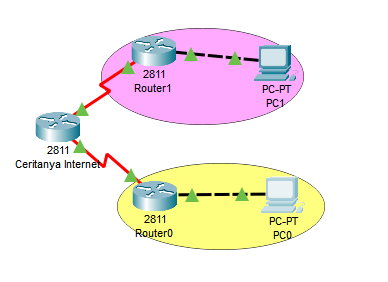
\includegraphics[width=0.5\linewidth]{tumod/tumod topologi p5.png}
  \caption{Hasil Topologi}
  \label{fig:topologi tumod}
\end{figure}

    \item Hasil pengujian konektivitas (ping test antar PC).
\begin{figure}[h]
  \centering
  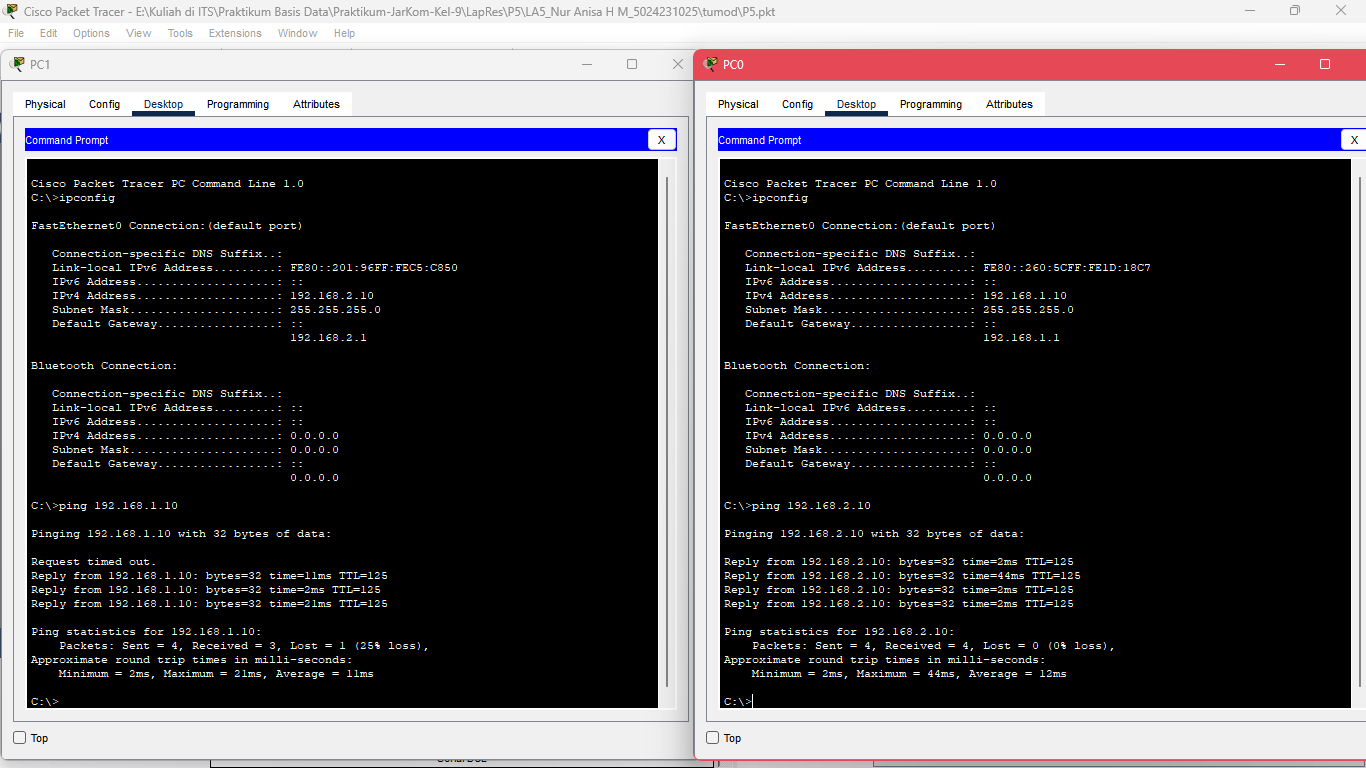
\includegraphics[width=0.5\linewidth]{tumod/ping.png}
  \caption{Hasil Tes Koneksi}
  \label{fig:topologi tumod}
\end{figure}  
  
    \item Penjelasan singkat tentang fungsi PPTP dalam jaringan tersebut.
    PPTP pada jaringan ini digunakan agar PC 0 dan PC 1 dapat saling berkomunikasi seakan-akan berada berada di network yang sama (tanpa routing).
  \end{itemize}
\end{enumerate}

\section{Kesimpulan}
Berdasarkan praktikum yang telah dilakukan, didapatkan beberapa kesimpulan penting. Pertama, Query cukup efektif dalam membatasi bandwidth dari koneksi. Kedua, VPN memang bisa digunakan untuk emmungkinkan koneksi langsung seakan-akan seperti koenksi lokal.

\section{Lampiran}
\subsection{Hasil Praktikum}
\begin{figure}[h]
  \centering
  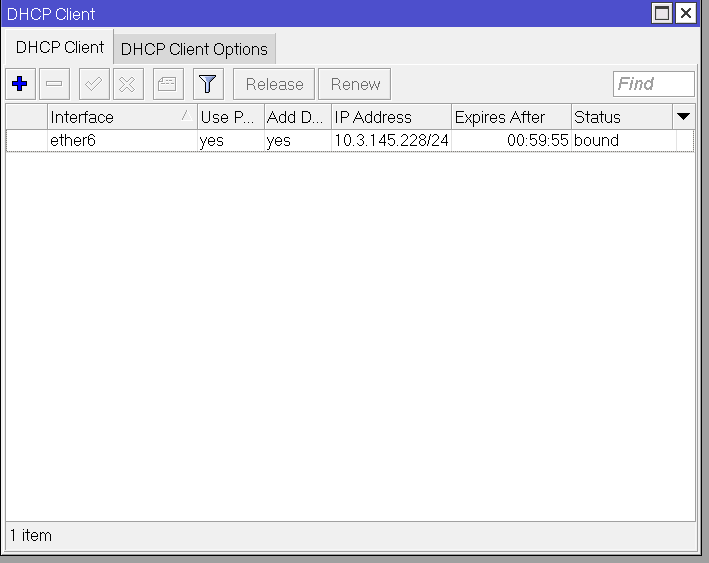
\includegraphics[width=0.5\linewidth]{dokum/Laptop 2/DHCP CLient.png}
  \caption{Hasil Konfigurasi DHCP Client}
  \label{fig:dhcp-client}
\end{figure}

\begin{figure}[h]
  \centering
  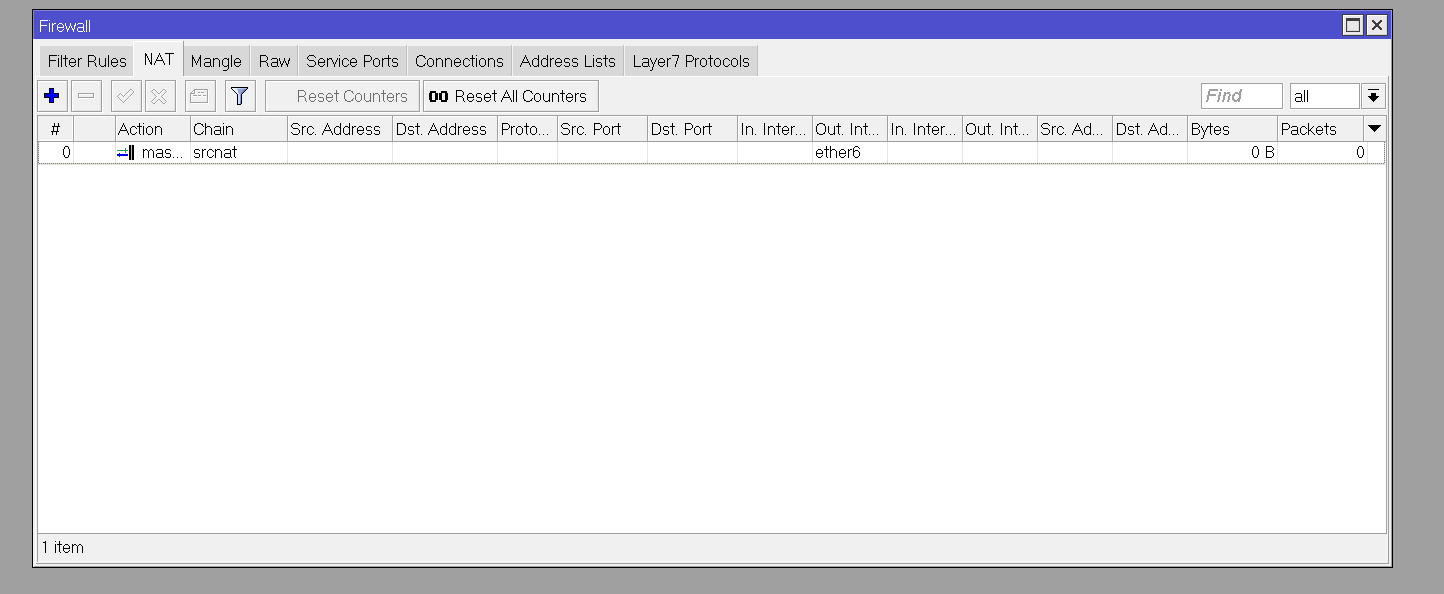
\includegraphics[width=0.5\linewidth]{dokum/Laptop 2/NAT.png}
  \caption{Hasil Konfigurasi NAT}
  \label{fig:nat}
\end{figure}

\begin{figure}[h]
  \centering
  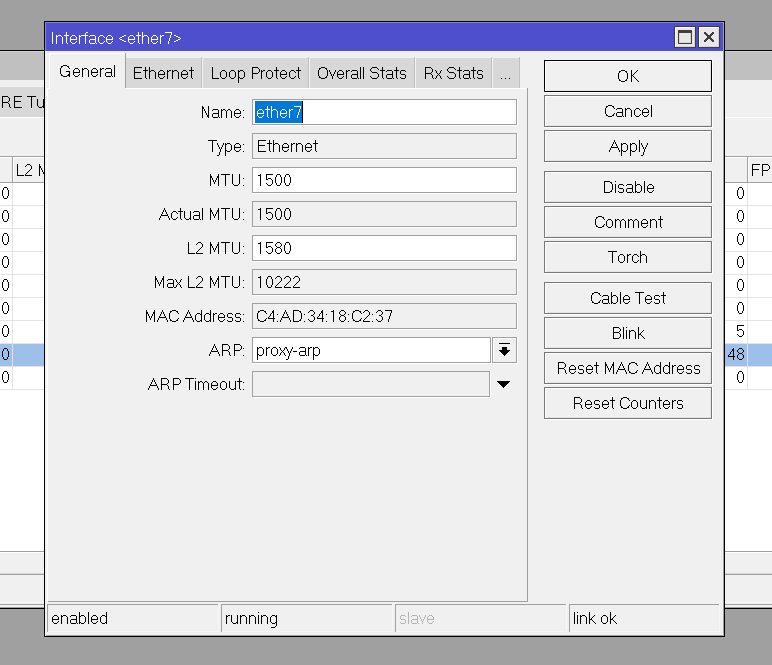
\includegraphics[width=0.5\linewidth]{dokum/Laptop 2/Screenshot 2025-06-05 162848.png}
  \caption{Hasil Konfigurasi IP}
  \label{fig:ip}
\end{figure}

\begin{figure}[htbp]
  \centering
  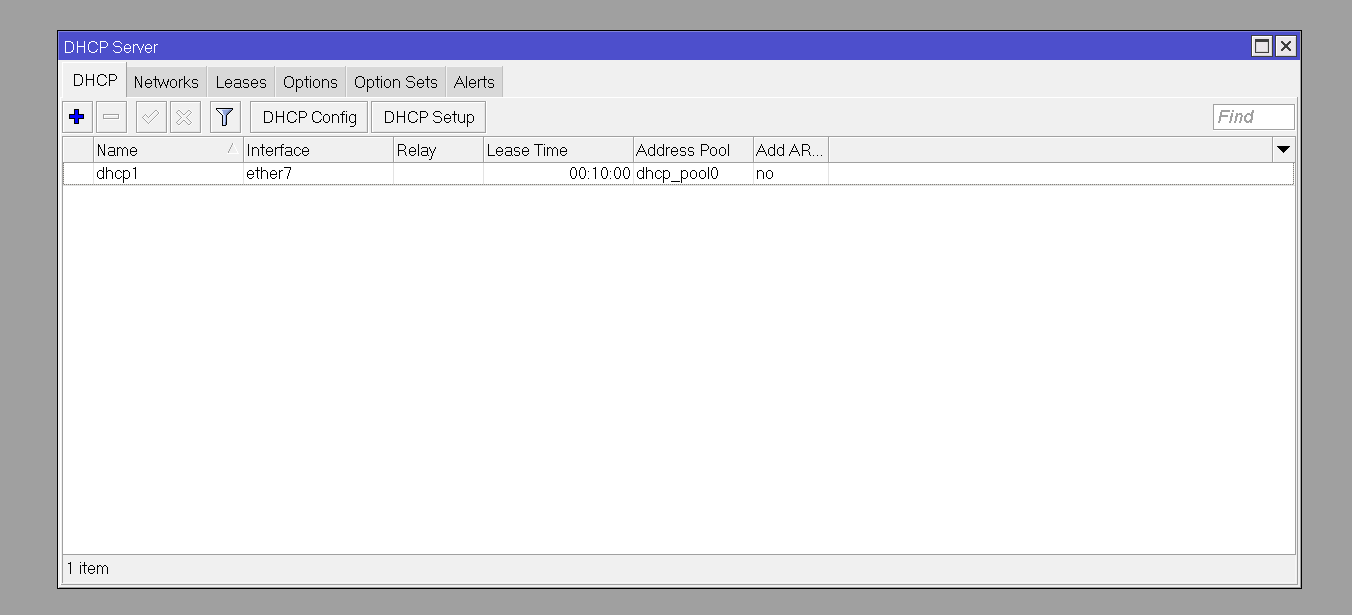
\includegraphics[width=0.5\linewidth]{dokum/Laptop 2/DHCP Server.png}
  \caption{Hasil Konfigurasi DHCP Server}
  \label{fig:dhcp-server}
\end{figure}

\begin{figure}[htbp]
  \centering
  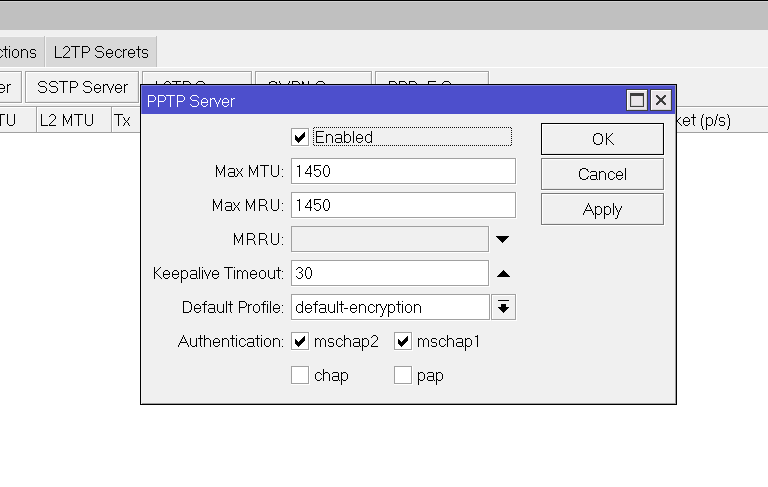
\includegraphics[width=0.5\linewidth]{dokum/Laptop 2/PPTPServer.png}
  \caption{Hasil Konfigurasi PPTP Server}
  \label{fig:PPTP-Server}
\end{figure}

\begin{figure}[htbp]
  \centering
  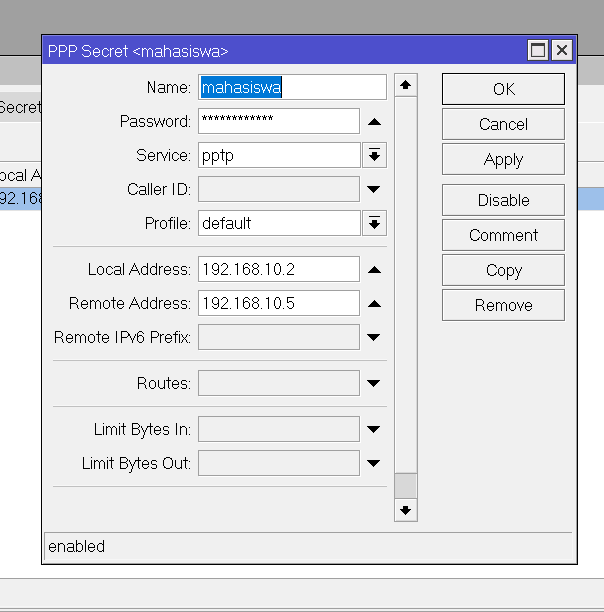
\includegraphics[width=0.5\linewidth]{dokum/Laptop 2/PAssword PPP.png}
  \caption{Hasil Konfigurasi User PPTP}
  \label{fig:pptp-user}
\end{figure}

\begin{figure}[htbp]
  \centering
  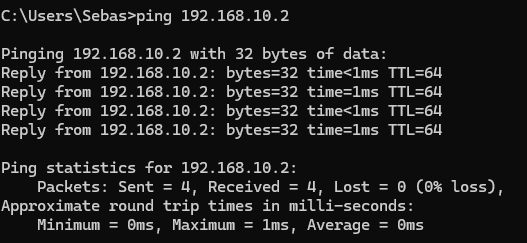
\includegraphics[width=0.5\linewidth]{dokum/ping server.png}
  \caption{Hasil Ping Server VPN}
  \label{fig:ping-vpn-server}
\end{figure}

\begin{figure}[htbp]
  \centering
  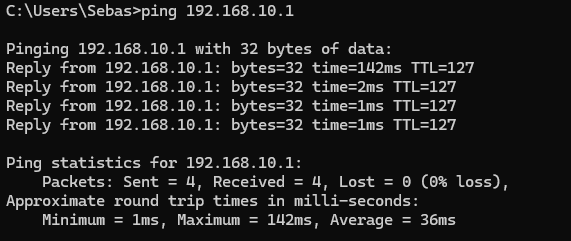
\includegraphics[width=0.5\linewidth]{dokum/ping pc2.png}
  \caption{Hasil Ping Laptop VPN}
  \label{fig:ping-vpn-laptop}
\end{figure}

\begin{figure}[htbp]
  \centering
  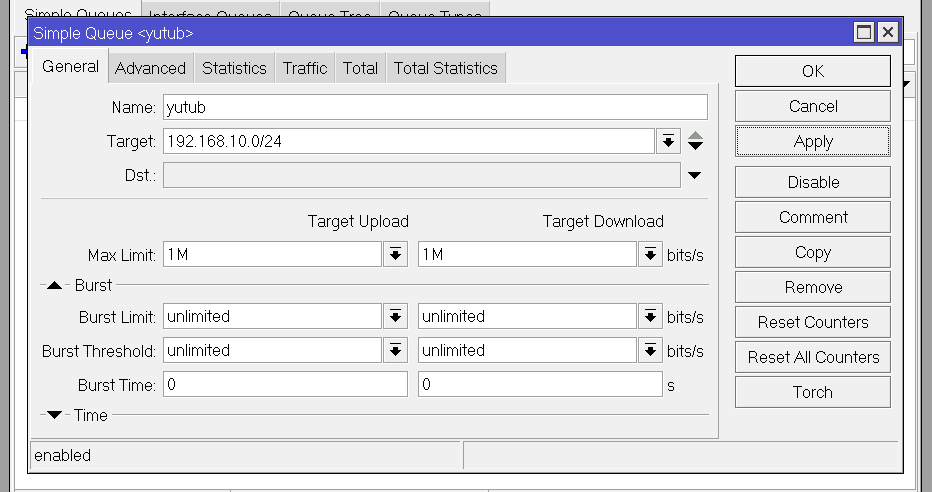
\includegraphics[width=0.5\linewidth]{dokum/Laptop 2/Simple Queq.png}
  \caption{Hasil Konfigurasi Simple Queue}
  \label{fig:queue}
\end{figure}

\begin{figure}[htbp]
  \centering
  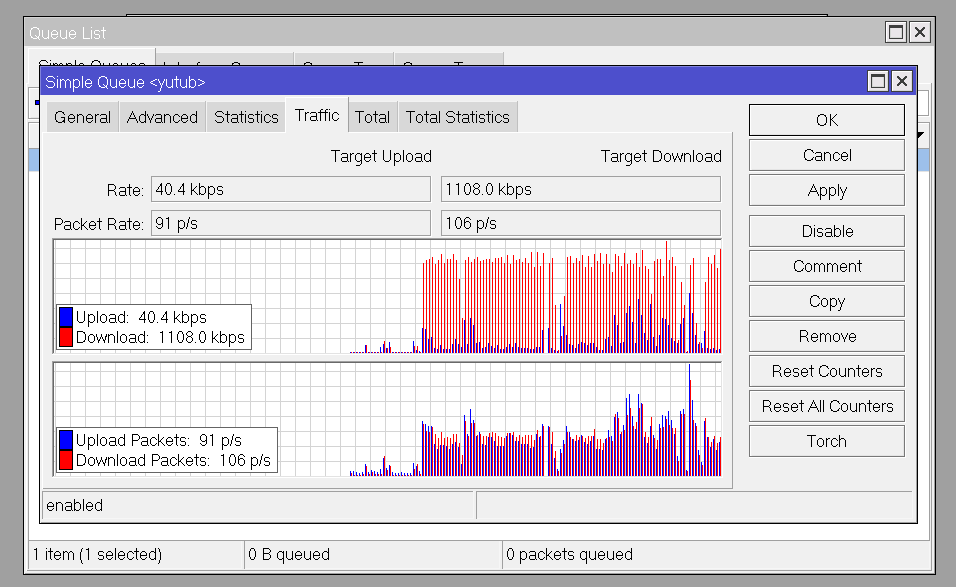
\includegraphics[width=0.5\linewidth]{dokum/Laptop 2/Grafik.png}
  \caption{Hasil Grafik Simple Queue}
  \label{fig:queue-grafik}
\end{figure}

\begin{figure}[htbp]
  \centering
  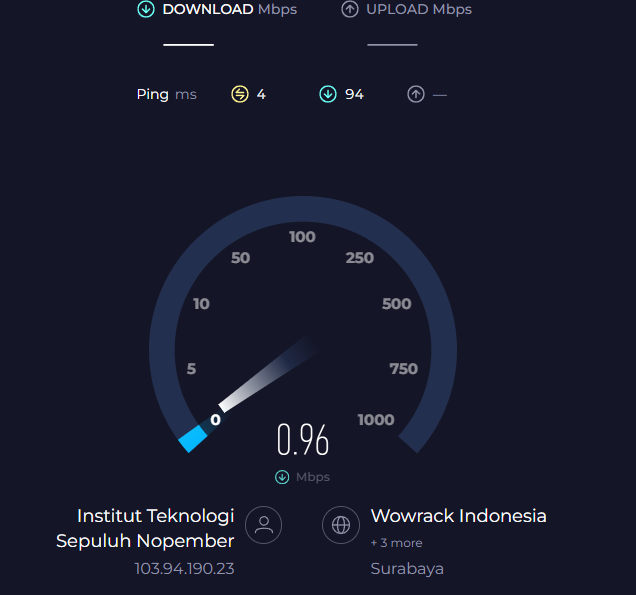
\includegraphics[width=0.5\linewidth]{dokum/speedtest.png}
  \caption{Hasil Speedtest saat Queue Aktif}
  \label{fig:test-aktif}
\end{figure}

\begin{figure}[htbp]
  \centering
  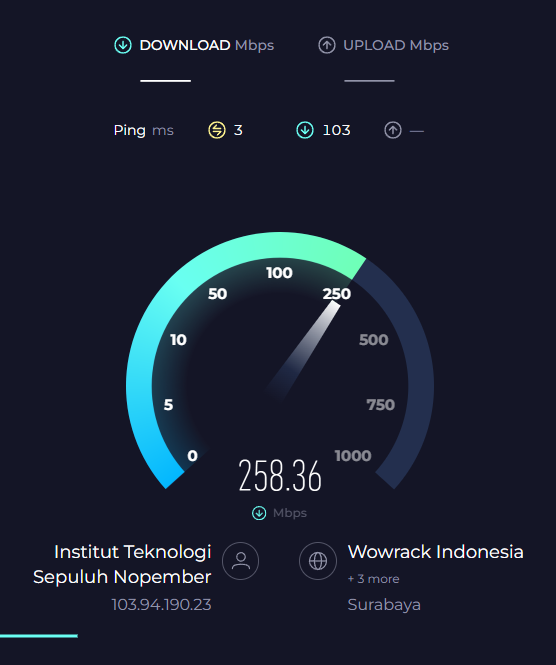
\includegraphics[width=0.5\linewidth]{dokum/speedtestlimit.png}
  \caption{Hasil Speedtest saat Queue Non Aktif}
  \label{fig:test-non-aktif}
\end{figure}

\subsection{Dokumentasi saat praktikum}
\begin{figure}[htbp]
  \centering
  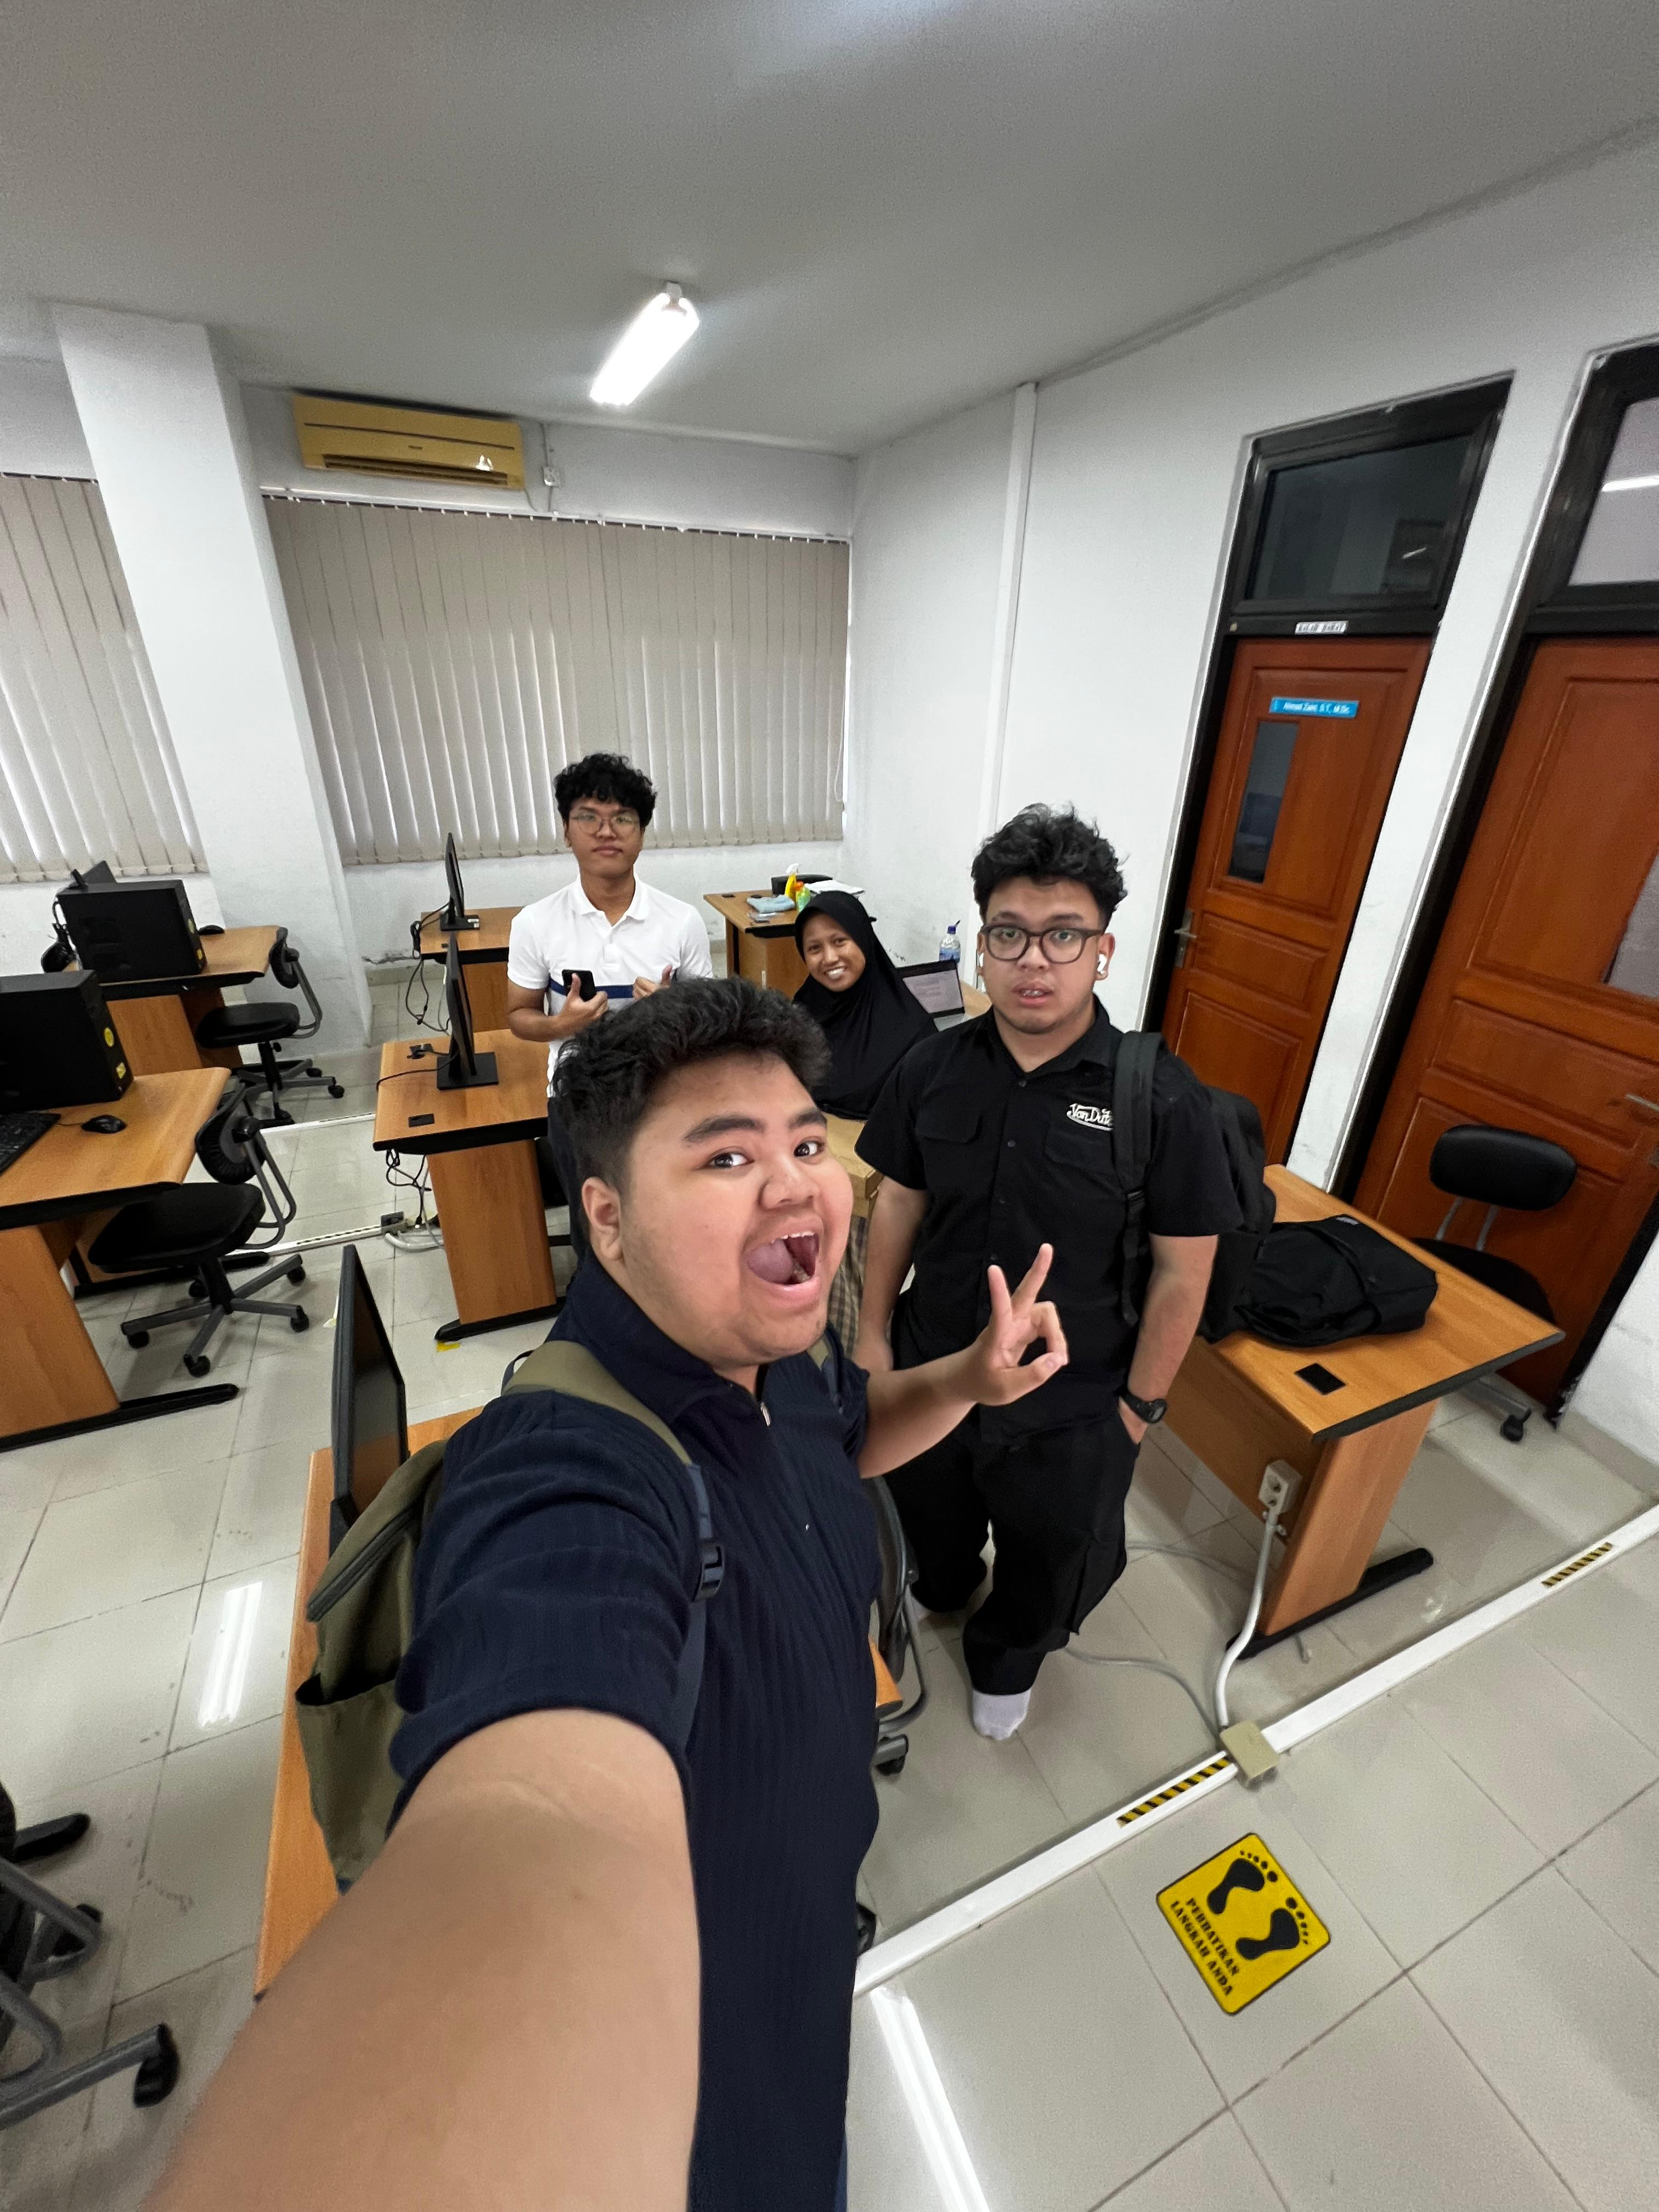
\includegraphics[width=.5\linewidth]{dokum/dokum.jpg}
  \caption{Dokumentasi Praktikum}
  \label{fig:dokum}
\end{figure}


